\documentclass[12pt,a4paper,openright,twoside]{book}
\usepackage[utf8]{inputenc}
\usepackage{disi-thesis}
\usepackage{code-lstlistings}
\usepackage{notes}
\usepackage{shortcuts}
\usepackage{acronym}
\usepackage{float}

\school{\unibo}
\programme{Department of Computer Science and Engineering - DISI\\Master's Degree in Digital Transformation Management}
\title{Design and Implementation of an Intelligent Call Routing System in the Banking Sector for Improved Customer Experience}
\author{Anna Campagna}
\date{\today}
\subject{Machine Learning}
\supervisor{Prof. Matteo Francia}
\cosupervisor{Dott. CoSupervisor 1}
\morecosupervisor{Dott. CoSupervisor 2}
\session{2nd}
\academicyear{2025-2026}

% Definition of acronyms
\acrodef{IoT}{Internet of Thing}
\acrodef{vm}[VM]{Virtual Machine}


\mainlinespacing{1.241} % line spacing in mainmatter, comment to default (1)

\begin{document}

\frontmatter\frontispiece

\begin{abstract}	
Max 2000 characters, strict.
\end{abstract}

\begin{dedication} % this is optional
Optional. Max a few lines.
\end{dedication}

%----------------------------------------------------------------------------------------
\tableofcontents   
\listoffigures     % (optional) comment if empty
\lstlistoflistings % (optional) comment if empty
%----------------------------------------------------------------------------------------

\mainmatter

%----------------------------------------------------------------------------------------
\chapter{Introduction}
\label{chap:introduction}
%----------------------------------------------------------------------------------------

Artificial intelligence (AI) refers to the development of computer
systems that can simulate human learning, problem solving, perception, decision-making, and
comprehension \cite{franken2019impact}. To be capable of all that, AI systems exploit various techniques,
including machine learning, deep learning, natural language processing,
and computer vision, to analyze large amounts of data and make predictions
or decisions based on that analysis \cite{malik2024artificial}.

In recent years, the use of artificial intelligence tools has rapidly escalated in all sectors of the economy, mainly thanks to the growing volume of digital data and higher computational capacity \cite{fernandez2019artificial}.
Malik et al., in their literature review on the industrial application of AI, report some examples of AI exploitation in different sectors:
\begin{itemize}
    \item in all sectors, AI-based intelligence and computer technologies can be exploited to create smart factories, which allow businesses to schedule advanced manufacturing lines and improve supply chain management reducing the risk for human errors;
    \item in the pharmaceutical sector, AI technologies accelerate research and development efforts in the identification and development of new pharmaceutical compounds to treat various medical conditions;
    \item in the e-commerce industry, AI enhance the consumer experience and increase sales for businesses by enabling personalized recommendations and targeted marketing strategies;
    \item in the automotive industry, AI enables autonomous driving, performs predictions on vehicle maintenance needs, and optimizes route computations.
\end{itemize}

As stated by Fernandez, using artificial intelligence techniques in the provision of financial services can heighten efficiency,
reduce costs, enhance quality, and raise customer satisfaction levels, as they allow to automate repetitive processes.
The banking sector in particular has become one of the most active adopters of AI, integrating it across customer-facing channels,
risk management, and back-office operations; a more detailed overview of these applications is provided in \cref{chap:state-of-the-art}.

In the context of customer support, one widely exploited AI application is the AI-based conversational agent,
which can simulate human conversations through voice commands \cite{zhang2023impact}.

\subsubsection{Case Study}
For one of their clients in the banking sector, Iriscube Reply S.r.l. had already implemented a conversational agent
capable of supporting customers for simple concerns such as bank transfers and common information requests.
The contact center otherwise follows the conventional Automatic Call Distribution (ACD)
architecture described in \cref{chap:state-of-the-art}: when a request falls outside what the conversational agent can handle,
the call is escalated and queued for a human operator, matched primarily on availability and coarse-grained routing rules rather
than on a fine-grained understanding of the customer's underlying need.
This is the baseline situation the project presented in this thesis aims to improve upon.

The designed and implemented intelligent call routing system has the objective of predicting the calling customer's
need based on their call history, their incomplete customer journeys on the home-bank application, their open tickets, and so on,
so that the call can be immediately routed to the most suited human operator.
The objective of this system is to increase the calling queue efficiency by assigning to each calling customer a priority score based
on their criticity and financial value, other than to improve the customer's experience.
\label{donne-ricche}

In fact, a natural first intuition is that customer dissatisfaction with call centers is primarily driven by long waiting times,
and that reducing wait times is therefore the main lever available to improve satisfaction.
However, this intuition is only partially supported by the literature.
In a survey of over three thousands customers of a telephone call center performed by Garcia et al.,
actual queue time was found to play a significant, but comparatively small, role in customers' overall time satisfaction.
Instead, the study found that the ability to keep customers satisfied while waiting depends much more on delivering
an informative, satisfactory answer along with a high standard of service, even when queue times are considerable \cite{garcia2012waiting}.
In other words, customers appear to tolerate some amount of waiting so long as the eventual interaction resolves their issue effectively.
This finding has an important implication for the design of call routing systems:
optimizing purely for shorter queues, without regard for whether the customer is subsequently connected to an operator capable of resolving their specific need,
addresses only part of the problem. A call answered quickly by an unsuitable operator may leave the customer no more satisfied
than a call answered slowly by a suitable one, and in the worst case, requires a second contact to actually resolve the issue,
having an impact on customers' frustration and, consequently, their churn risk.

This second contact, and its associated cost to both the customer's experience and the organization's efficiency,
is well studied under the concept of First Call Resolution (FCR): the ability of a contact center to resolve a customer's
request within a single interaction, without requiring the customer to call back for the same reason.
Empirical research based on a survey of 168 call center managers, has shown that FCR positively mediates the relationship between
knowledge management, technology-based customer relationship management (CRM) systems, and caller satisfaction within inbound contact centers \cite{abdullateef2011mediating}.
This provides direct empirical support for the intuition motivating this thesis: a call that is routed to an operator who cannot resolve the customer's actual need
is unlikely to be satisfactorily closed on the first attempt, regardless of how quickly that operator was reached.

Crucially, both the technology-based CRM component and the knowledge-management component identified as antecedents of FCR in this line of research
are directly relevant to the system proposed in this thesis, which aggregates CRM signals (call history, incomplete application journeys, open tickets)
specifically in order to better inform the routing decision at the moment of the call.

A parallel stream of research has examined how the human, employee-side factors of a call center interaction shape customer satisfaction,
independently of purely operational metrics such as queue length. Drawing on Service Quality, Human Resource Management, and Marketing literature,
an empirical study covering 109 call centers found that employee-related variables meaningfully contribute to the paths that lead to customer satisfaction in call center settings \cite{chicu2019exploring}.
This supports the idea, central to this thesis's problem framing, that \emph{who} answers a call is not incidental to the customer's experience of that call:
an operator whose skills, experience, or specialization do not match the customer's actual need represents a structural risk to satisfaction,
independent of how efficiently the call center's queueing mechanism performed.

The broader operational challenge of assigning heterogeneous incoming requests to a heterogeneous pool of operators has long been recognized as a core problem
in call center operations research. Call centers have been described as a fertile area for operations management research spanning forecasting, capacity planning,
queueing, and personnel scheduling \cite{aksin2007modern}. Within this tradition, skill-based routing has been studied as a way to move beyond simple
availability-based assignment: because it is generally not possible or cost-effective to train every operator to handle every type of request,
operators tend to have different skills in different combinations, which makes routing calls effectively, and determining adequate staffing levels,
a genuinely difficult problem \cite{wallace2005staffing}. Existing skill-based routing approaches, however, typically rely on explicitly defined and
manually maintained operator skill profiles matched against a coarse classification of the incoming request (e.g., by department or declared topic),
rather than on a prediction of the customer's specific intent derived from their historical behavior across multiple channels.


\paragraph{Structure of the Thesis}
This thesis will be structured as follows. First, the state of the art about the usage of AI in banking, Automatic Call Distribution systems, and conversational agents will be presented. Then follows a presentation of the analysis of requirements, of the system's design, and of the implementation. Finally, a thorough evaluation of the system will be performed.

The remainder of this thesis is organized as follows.

\cref{chap:state-of-the-art} presents the state of the art relevant to this work, covering the exploitation of AI in the banking sector,
the operation of traditional Automatic Call Distribution systems, the design of LLM agents and conversational agents,
literature's contribution to the intent classification and skill-based routing problems.

\cref{chap:design} and \cref{chap:implementation} present, respectively, the design and implementation of the proposed system,
covering both the traditional machine learning pipeline and the agentic LangGraph-based pipeline,
including the architectural decisions specific to each.

\cref{chap:evaluation} presents ............

Finally, \cref{chap:conclusion} summarizes the contributions of this thesis, discusses their limitations,
and outlines future directions.

\chapter{State of the art}
\label{chap:state-of-the-art}


\section{AI Exploitation in Banking}

Banks are considered as the life blood of an economy as it handles cash, credit and financial transactions. To cut down the operating expenses and to improve the efficiency, the banking sector is adopting updated technologies like AI, cloud and block-chain. Moreover, digitalization is rapidly growing and influencing banks to adopt new technologies for better customer service.

AI is currently exploited in the banking sector for the following applications \cite{kochhar2019rise}, \cite{jain2023role}:
\begin{itemize}
    \item \textbf{Data Analytics}: data analytics is of great assistance, as patterns of customer behavior can be observed by quick processing of data and banks can predict the future outcomes. Hence, banks can contact the customer at the right time with the right product. Data analytics can be used not only for products and services customization, but also for fraud prevention, credit scoring, investment management, and more.
    \item \textbf{Customer Relationship Management}: chatbots help in understanding the customer and responding in a correct manner. They are automated communication channels, therefore they are available 24/7 and improve the relationship with customers.
    \item \textbf{Robotic Process Automation (RPA)}: automation of repetitive, rule-based digital tasks, such as data entry, document verification, and compliance checks, which traditionally required manual intervention.
\end{itemize}

Artificial Intelligence is so important to the banking sector as it helps banks work in a more efficient and effective manner. Jain further notes that AI-driven systems allow banks to process significantly larger volumes of transactions and customer interactions than traditional rule-based systems, while simultaneously reducing the operational cost per interaction \cite{jain2023role}.

On the strictly financial side, the advantages of AI usage for banks are:
\begin{itemize}
    \item Cost reduction, as it helps customers in performing their own activities, speed-up response time, handling the data with accuracy, and many more;
    \item Revenue increase, thanks to increased employee effectiveness, as part of their tasks can be automated by RPA.
\end{itemize} 
On a more operational note, AI represents a competitive advantage for banks in:
\begin{itemize}
    \item Investment management, as AI algorithms can make informed investment decisions by analyzing vast amounts of market data, historical trends, and news;
    \item Risk mitigation, as many banks are using AI to protect themselves and their customers from fraud and cyber risks;
    \item Customer satisfaction, which increases as a consequence of process automation, as customers get the responses they are looking for faster;
    \item Credit decisions and loan eligibility evaluation, where machine learning models are trained on historical repayment behavior and financial indicators to estimate default risk more accurately and consistently than traditional scorecards, and to shorten loan origination times;
    \item Fraud detection, as the great amount of data generated by the thousands of transactions that take place daily allow to identify patterns and anomalies in customers' behaviors.
\end{itemize}

In summary, for a bank to keep its competitive advantage, AI integration is fundamental. While navigating through banking sites, customers tend to ask a set of common questions which can be answered in an effective way with AI applications. Customer service is found to be the most popular use-case for chatbot assistance: by automating responses to frequent, low-complexity requests, banks are able to increase customer engagement while also strengthening their brand image \cite{bhattacharya2022role}. This trend towards automated, always-available customer service channels is precisely what motivates the next section, which examines in more detail how contact centers route the requests that cannot be resolved by such automated channels.

\section{Automatic Call Distribution Systems}

An Automatic Call Distributor (ACD) is part of the telephony-switch infrastructure in a call center \cite{listova2018formation}. It collects operational data, such as each call's arrival time, waiting time in a telephone queue, and duration of service, and it acts as a switch routing the call to an operator, while keeping trace of every call's history as it flows through the contact center.

ACDs are designed to streamline incoming call handling, following the process shown in \cref{fig:ACD} \cite{Nice-ACD};
\begin{enumerate}
    \item The ACD identifies the caller's need using tools like Interactive Voice Response (IVR);
    \item Based on the identified need, the system matches the caller to the best operator;
    \item If all agents are busy, the caller is placed in a queue and the system monitors wait times and manages call prioritization based on urgency or customer's importance;
    \item Once an agent becomes available, the system assigns the next call in queue ensuring fair workload and quicker customer service.
\end{enumerate}

\begin{figure}[H]
    \centering
    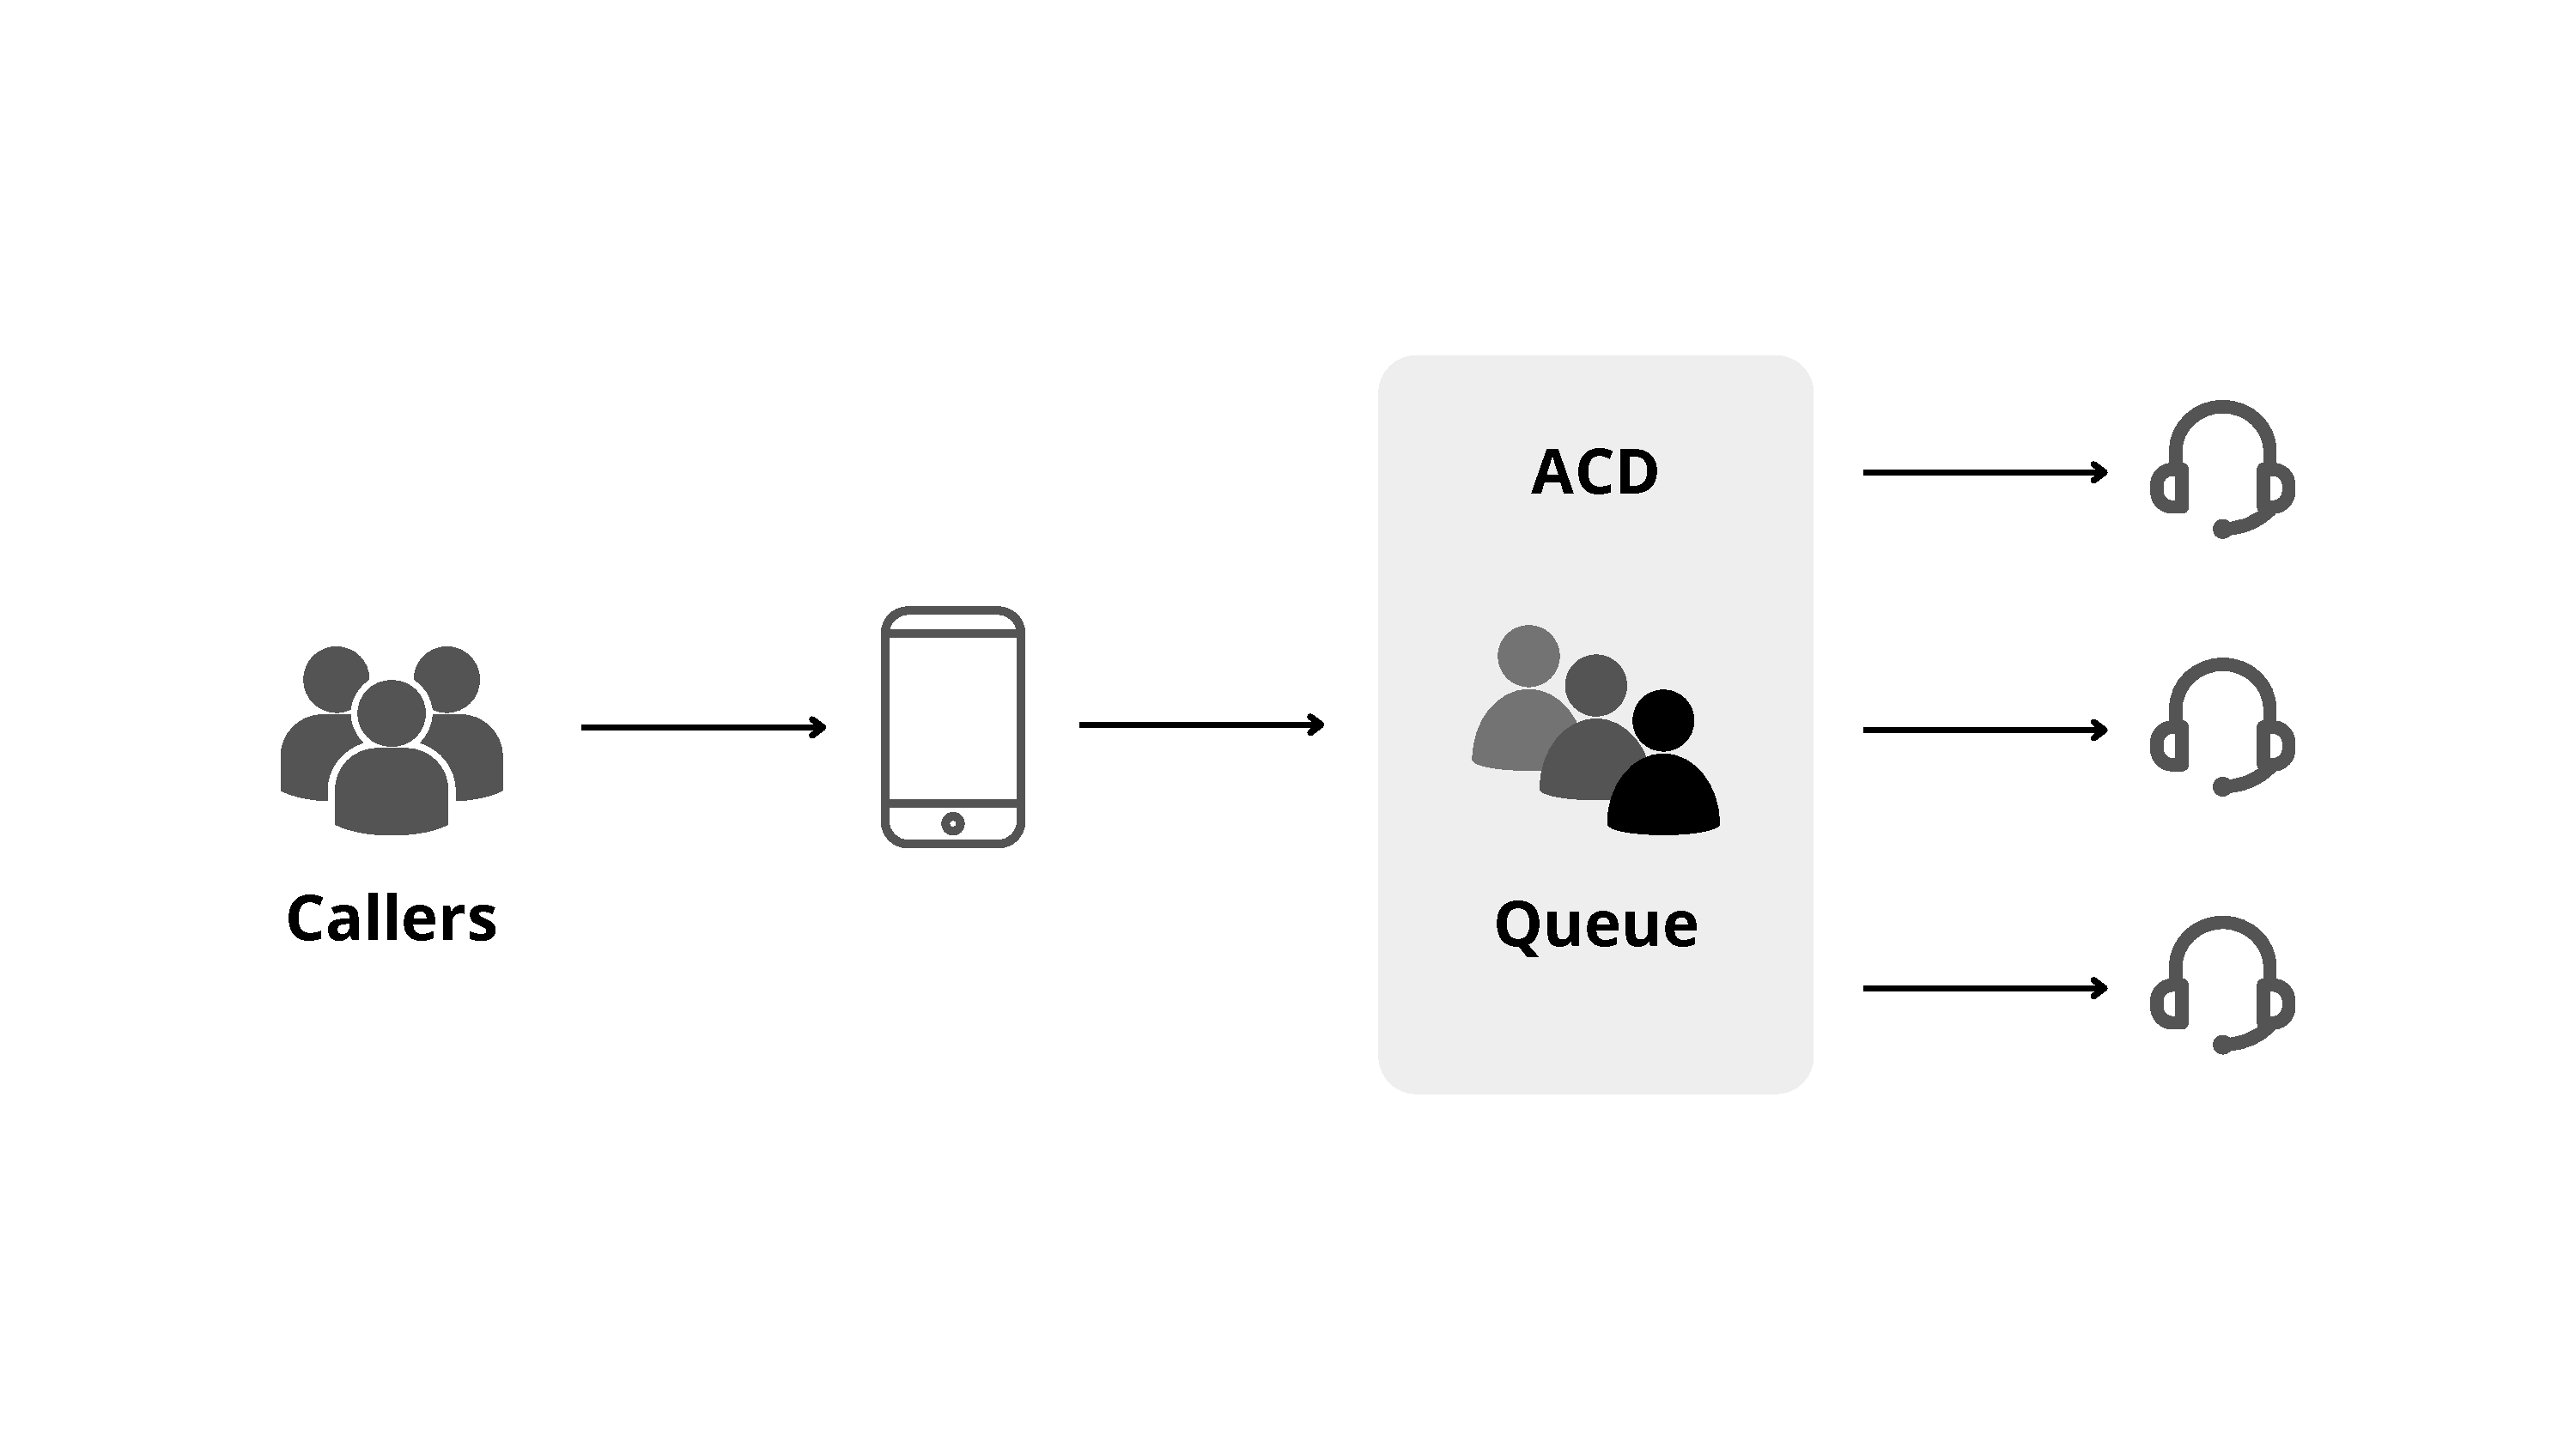
\includegraphics[width=.8\linewidth]{figures/ACD.pdf}
    \caption{Automatic Call Distribution system flow}
    \label{fig:ACD}
\end{figure}

The above-mentioned IVR is a recorded interactive script that allows the caller to receive and provide information
or make requests by pressing the keys of a touch telephone \cite{corkrey2002interactive} or their voice \cite{gans2003telephone}.
Typically, 3 types of IVR systems can be found \cite{IBM-IVR}:
\begin{itemize}
    \item Touch-tone replacement: the caller is asked by a pre-recorded message to use a keypad selection to access information. For example, "Press one for account balances", "Press two for recent transactions", "Press three to transfer money", and the user is expected to press the key corresponding to their need;
    \item Directed dialog: it provides specific verbal prompts to the caller depending on their inquiry. For example, the recording might ask "Do you want to know about account balances or about recent transactions?" and the caller can respond with "Recent transactions";
    \item Natural language: it uses speech recognition to better understand user requests. For example, the system prompt can generically ask "What information are you looking for today?", and the caller may reply with "I want to know my recent transactions".
\end{itemize}

IVRs can also be used to direct the call center's computers to provide simple services,
such as the transfer of funds among bank accounts \cite{gans2003telephone}.
In fact, Gans et al. report that in many banking call centers
about 80\% of customer calls are fully self-served using an IVR.

\section{LLM Agents and Agentic Architectures}
\label{sec:llm-agents}
AI research is currently undergoing a shift away from passive, task-specific tools and toward autonomous
systems endowed with genuine agency \cite{DBLP:journals/air/AliDC26}. Unlike conventional AI models,
which passively respond to queries or execute predefined tasks, agentic AI systems actively plan, coordinate,
and act upon their environment in pursuit of longer-term goals \cite{DBLP:journals/air/AlvaP26}.

Abou Ali et al. define an AI agent (or single-agent system) as a self-contained, autonomous system built to pursue
a specific goal, typically operating on its own even when it draws on external tools and APIs. What makes it agentic
is the combination of autonomy, proactivity, and the capacity to carry a task through to completion without ongoing human guidance \cite{DBLP:journals/air/AliDC26}.
Here, autonomy denotes the system's capacity to act independently of direct human intervention, whereas agency refers
more specifically to goal-directed behavior, encompassing intention, awareness of context, and decision-making.

Agentic AI, by contrast, denotes the wider field and architectural paradigm concerned with building systems that display
this kind of agency. It brings autonomy and agency together into systems that can initiate their own tasks, reprioritize
goals on the fly, track their own progress, and revise their behavior in response to feedback.

The vocabulary used to describe agency today has roots in the earlier symbolic paradigm, built around explicit logical rules,
algorithmic planning, and deterministic or probabilistic models \cite{DBLP:journals/air/AliDC26}. Under symbolic reasoning,
intelligence was essentially reduced to the manipulation of human-readable symbols: systems relied on hand-coded rules and
knowledge bases, which made their behavior transparent but also rigid and devoid of genuine agency \cite{DBLP:journals/access/MorallesCRKSSPSR26}.
A significant step forward came with the Belief-Desire-Intention (BDI) architecture, which formalized agency by giving
agents internal representations of the environment (beliefs), objectives to pursue (desires), and committed courses of action (intentions),
effectively bridging symbolic logic with agent-oriented programming. BDI agents could reason about possible future states
and adjust accordingly, yet they remained tied to symbolic representations and tended to be brittle once deployed in uncertain
or unstructured settings \cite{DBLP:journals/access/MorallesCRKSSPSR26}.

More recently, this symbolic paradigm has given way to a neural one \cite{DBLP:journals/air/AliDC26}:
AI has progressed over the past decades from rule-based expert systems, through learning-based methods,
to today's large language models (LLMs) \cite{DBLP:journals/apin/Gabauer26}.
This neural lineage rests on statistical learning from data and culminates in the generative capabilities
now exhibited by LLMs \cite{DBLP:journals/air/AliDC26}. Within this landscape, modern agentic architectures
can be grouped into three broad categories \cite{DBLP:journals/access/MorallesCRKSSPSR26, DBLP:journals/air/AliDC26, DBLP:journals/apin/Gabauer26}:

\begin{itemize}
    \item \textbf{Multi-Agent Systems}, in which several agents operate within a shared environment and interact through
    coordination (synchronizing their actions), cooperation (pursuing common goals), negotiation or competition (resolving conflicting interests).
    An orchestrator, frequently an LLM itself, plays the role of context manager and task router, evaluating the overall objective and distributing
    specialized subtasks among the other agents accordingly;
    \item \textbf{Reinforcement Learning Agents}, which learn through trial-and-error interaction with their environment,
    progressively updating their policy to maximize cumulative reward;
    \item \textbf{LLM-based Agents}, which rely on natural language as their primary interface and are capable of tackling
    complex tasks by combining planning, external tool use, and multi-step reasoning.
\end{itemize}

A number of frameworks have emerged that attempt to operationalize agentic AI by integrating LLMs with planning and action-execution mechanisms \cite{DBLP:journals/air/AlvaP26};
their main contribution generally lies in how they handle dynamic context management, prompt engineering, and the composition of external tools \cite{DBLP:journals/air/AliDC26}.
Some of the most relevant examples proposed by Alva et al. are outlined below.

\begin{itemize}
    \item \textbf{LangChain} is a loosely coupled, highly customizable framework for building LLM-powered applications
    by composing prompts, tools, and memory components. It integrates well with vector stores, external APIs, and function-calling mechanisms,
    but does not natively support autonomous goal decomposition or real-time feedback loops. % DETTAGLIO RILEVANTE
    \item \textbf{AutoGPT} was among the first open-source systems to demonstrate one of the defining capabilities of LLMs:
    reasoning about, planning, and executing a sequence of tasks. It structures agent behavior as a recursive loop in which
    the LLM is repeatedly prompted to reflect on the current step, plan the next one, and act accordingly.
    However, it lacks a realistic representation of state and environmental awareness, which makes it unreliable on long-horizon tasks.
    \item \textbf{ReAct} introduced a paradigm that interleaves verbal reasoning with concrete actions: the agent articulates
    intermediate reasoning steps, issues API calls, and adapts its subsequent behavior based on the outcome. Its scope, however, remains largely confined
    to prompt-engineering patterns, without built-in support for persistent memory or coordination across multiple agents.
    \item \textbf{CrewAI} provides an infrastructure for decomposing a task among specialized agents and integrating their individual outputs into
    a shared workflow, but it lacks standardized mechanisms for state sharing, hierarchical planning, and goal alignment,
    all of which are needed to build scalable and robust agentic applications.
\end{itemize}

\section{Conversational Agents}
\label{sec:conversational-agents}

Conversational agents, dialogue systems, and virtual assistants are some of the terms that can be found
in scientific literature to describe software-based systems capable of processing
natural language data to simulate a smart conversational process with humans \cite{motger2022software, balaraman2021recent}.
Existing dialogue systems are generally divided into task-oriented and non-task-oriented, according to their application \cite{chen2017survey}:
\begin{itemize}
    \item Task-oriented dialogue systems enable users to accomplish specific tasks,
    such as ticket booking, restaurant reservation, and customer support, by interacting in natural language.
    \item Non-task-oriented systems interact with humans to provide reasonable responses and entertainment,
    they typically focus on conversing with human on open domains.
\end{itemize}
Since the main interest of this work are task-oriented dialogue systems, only these will be explored in more detail.

A typical task-oriented dialogue system consists of \cite{gao2018neural} (\cref{fig:task-oriented}):
\begin{enumerate}
    \item A natural language understanding (NLU) module for identifying intents of user utterances;
    \item A dialogue state tracker (DST) for tracking conversation state;
    \item A dialogue policy which selects the next action based on the current state;
    \item A natural language generator (NLG) for converting the agent action to a natural language response.
\end{enumerate}

\begin{figure}
    \centering
    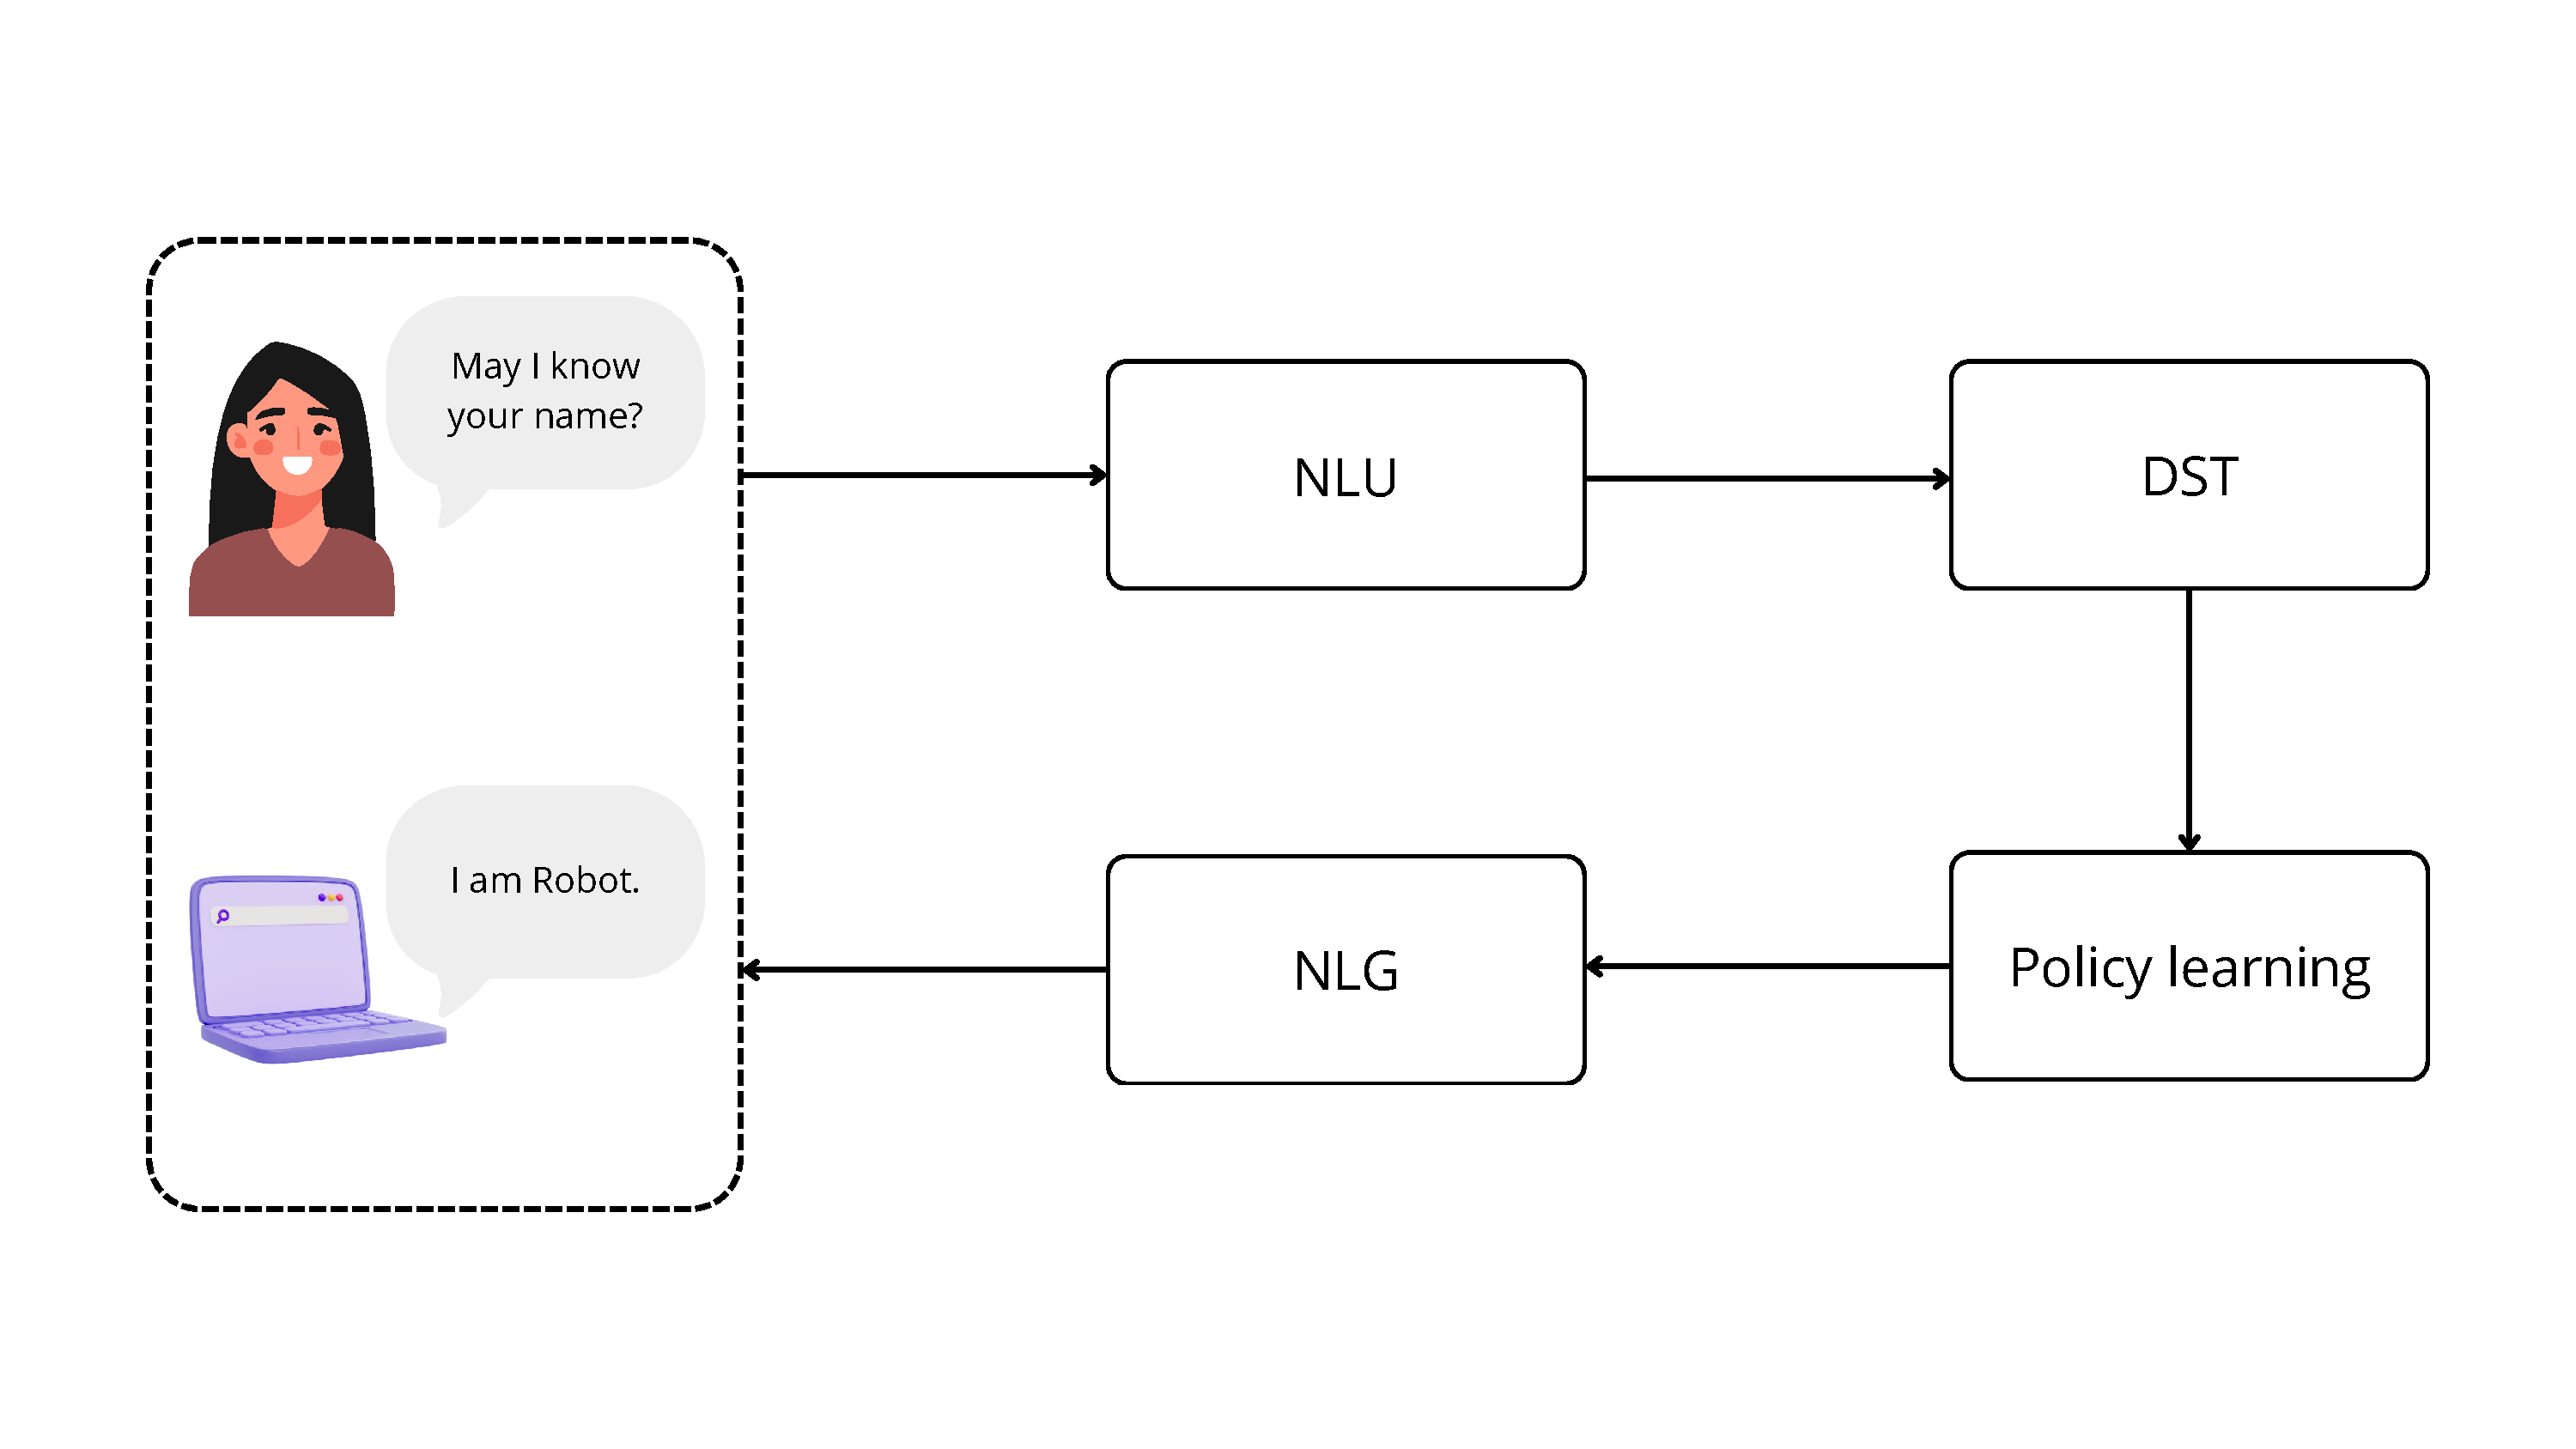
\includegraphics[width=.8\linewidth]{figures/task-oriented dialogue systems.pdf}
    \caption{Traditional pipeline for task-oriented systems}
    \label{fig:task-oriented}
\end{figure}

\subsection{Natural Language Understanding}
The NLU module maps a user utterance onto a set of predefined semantic slots.
Two complementary sub-tasks are typically involved: intent detection, which classifies the whole utterance
into one of a predefined set of intents, and slot filling, which extracts word-level information such as named entities,
and assigns a semantic label to each word or span in the utterance \cite{chen2017survey}.
For example, in the utterance "show restaurant at New York tomorrow", intent detection would classify the overall request
as a restaurant search, while slot filling would separately tag "New York" as a location and "tomorrow" as a date.
While early deployed systems relied primarily on manually crafted rules and features for both sub-tasks, deep learning
approaches have since been applied successfully to both intent detection and slot filling, learning feature representations
directly from data rather than from hand-crafted rules \cite{chen2017survey}.

\subsection{Dialogue State Tracking}
Once the user's utterance has been parsed by the NLU module, the dialogue state tracker is responsible
for maintaining an up-to-date summary of the conversation, known as the dialogue state, which contains
all the information the system needs to choose its next action \cite{balaraman2021recent}.
The dialogue state is typically represented as a set of slot-value pairs capturing the user's goal
as it has emerged over the conversation so far, and it can be updated in one of two ways:
turn-level prediction, where the model infers only the slot-values expressed in the current turn and then merges
this with the previous state through a separate update mechanism, or dialogue-level prediction,
where the model re-infers the complete state at every turn directly from the full conversation history \cite{balaraman2021recent}.

It is worth noting that, while DST is conventionally framed as a turn-by-turn process within a single spoken conversation,
the underlying problem it addresses, maintaining an evolving belief about what the user actually wants based on all information observed so far,
is conceptually close to the problem addressed by the system proposed in this thesis.
Rather than tracking a state across turns within one call, this thesis aggregates a customer's state across
multiple channels and past interactions prior to the call itself, effectively performing a form of state tracking
at the level of the customer's broader relationship with the bank rather than within a single dialogue session.

\subsection{Dialogue Policy Learning and Natural Language Generation}
Conditioned on the state produced by the DST module, the dialogue policy is responsible for selecting the next system action.
Both supervised learning, typically used to warm-start the policy from rule-based demonstrations, and reinforcement learning,
used to further optimize the policy toward long-term dialogue success rather than only the immediate next action, have been applied to this task \cite{chen2017survey}.
Finally, the natural language generation module converts the abstract action selected by the policy into a natural language surface utterance,
a step for which conventional approaches typically separate sentence planning from surface realization, while more recent neural approaches
condition the generation directly on the action type and its associated slot-value pairs \cite{chen2017survey}.

\subsection{Limitations of the Pipeline Architecture}
Despite being widely deployed, the traditional pipeline architecture presents two structural limitations \cite{chen2017survey}.
The first is the credit assignment problem: because the end user's feedback is only observed at the end of the interaction,
it is difficult to propagate this signal back to each individual upstream module (NLU, DST, policy, NLG) to determine which component
was responsible for a poor outcome. The second is process interdependence: since the input of each component depends directly on the
output of the previous one, adapting or retraining any single module to a new domain or with new data generally requires the other
modules to be adapted accordingly to preserve overall system coherence, which demands significant manual effort.
These limitations have motivated a shift toward end-to-end trainable architectures and, more recently, toward the agentic,
LLM-based architectures discussed in \cref{sec:llm-agents}, which reduce the reliance on tightly coupled, independently optimized pipeline stages.

\subsection{Emotion and Sentiment Recognition}
Beyond the core pipeline, some works propose extending conversational agents with a dedicated module for emotion and sentiment recognition,
enabling the system to assess the user's current emotional state in addition to the content of their query, and to select its response accordingly \cite{bertero2016real}.
Bertero et al. show that a convolutional neural network operating directly on raw audio, without any hand-crafted feature engineering,
can classify user emotion into six categories with an average accuracy of 65.7\%, outperforming a conventional feature-based Support Vector Machine baseline,
while a separate CNN-based sentiment classifier trained on textual transcriptions reaches an F-score of 82.5 when trained on out-of-domain data \cite{bertero2016real}.
In such architectures, the dialogue management component takes both the emotion/sentiment signal and the query content into account when deciding the appropriate response,
allowing otherwise conventional dialogue systems to react with a degree of empathy toward the user.

\section{Intent Classification}

Intent classification is the process of classifying user input text
or natural language utterances into one or more predefined intent
categories based on the domains and intents involved \cite{celikyilmaz2011exploiting, al2022intent}.

Intent detection from historical behavioral sequences is crucial for
enhancing recommendation accuracy and understanding consumer decision-making
processes from an economic perspective \cite{jin2025hicore}.
Moreover, it is fundamental in dialogue systems as it allows the system
to understand what the user wants to do, especially in systems where multiple
users with different goals are interacting with the system simultaneously \cite{al2022intent}.

Intent classification is particularly important for businesses because it
allows them to be more customer-centric \cite{al2022intent}, enabling platforms
to better match consumer needs, optimize market offerings, and potentially
increase consumer surplus \cite{jin2025hicore}.

This is especially true in customer support and sales areas, where faster response
times and personalized service can make a big difference with customers satisfaction,
as already explored in \cref{chap:introduction}.
Each customer has a specific purpose such as buying something,
asking a question, getting more information, or unsubscribing;
therefore it is crucial to understand the intention behind customer queries and
promptly respond to customers to improve satisfaction, retention rates, and loyalty \cite{al2022intent}.

However, training intent classifiers are often impeded by challenges such as
limited labeled data availability and the high cost associated with human labelers \cite{benayas2024enhancing}.
Data augmentation techniques aim to overcome this limitation by artificially
expanding the training dataset and introducing variations in the input text to
expose the model to a broader range of linguistic patterns.
LLMs play a central role in data generation and augmentation;
their generation process is heavily influenced by prompts input text that guides it.
The two main techniques are \cite{benayas2024enhancing}:
\begin{itemize}
    \item Fewshot technique: it involves designing a prompt with minimal examples of
    a particular task, and passing it to the LLM, enabling it to generalize to new,
    unseen examples with only a few instances provided;
    \item Zero-shot technique: it takes a step further than fewshot by prompting
    a model to perform tasks it has never seen during training.
\end{itemize}

Leveraging these approaches with LLMs enables effective adaptation to specific intent
classification tasks with limited labeled data \cite{benayas2024enhancing}.

Beyond the availability of labeled examples, the choice of architecture itself has
a substantial effect on intent classification performance in settings where the
target language or domain is poorly resourced. Purely transformer-based
encoders capture rich contextual information but do not always exploit the
sequential and morphological regularities present in languages with complex
inflection or non-standard orthography. To address this, recent work has
combined a domain-adapted transformer encoder with recurrent layers and an
attention mechanism on top, so that contextual embeddings are further refined
through sequential modeling before classification \cite{shafeeq2026rahbar}. In such hybrid designs, a
bidirectional recurrent component is stacked after the transformer to capture
short- and long-range dependencies between tokens, an attention layer is used
to weight the most discriminative parts of the utterance, and a final
transformer encoder layer is applied to the attention-refined representation
before the classification head. This layered combination has been shown to
outperform both the transformer encoder alone and conventional recurrent
baselines on a domain-specific, low-resource intent classification benchmark,
while also supporting post-hoc explainability techniques (such as LIME) that
surface the tokens most responsible for a given prediction \cite{shafeeq2026rahbar}.
This is particularly relevant for customer-facing systems, such as banking contact
centers, where the ability to justify an automatic routing or classification
decision to a human operator can be as important as raw accuracy.

The data augmentation and few/zero-shot strategies discussed above generally
assume that training examples are either confirmed positives or entirely
unlabeled. In deployed customer support systems, however, the composition of
available data is typically more nuanced. Human operators are commonly asked
only to confirm or reject a model's intent prediction, rather than to assign
a correct label when the prediction is wrong; this produces a mix of
confirmed positive cases, confirmed negative cases (i.e., hard, high-confidence
mispredictions with no explicit correct label), and a much larger volume of
uncurated cases that never receive human feedback at all \cite{dong2021semi}.
Treating the negative cases as discardable, or requiring them to be manually
reassigned to a class, both waste a valuable source of signal about the decision
boundary between intents. An alternative is to explicitly model the negative
feedback as a set of per-class binary classification tasks trained jointly
with the main multiclass objective, sharing a common encoder, so that the
confirmed negatives shape the decision boundary of the class they were
mistakenly routed to without needing a corrected label. Combined with an
iterative semi-supervised procedure that adds high-confidence predictions on
the uncurated data back into training, and with domain- and task-adaptive
pretraining of the encoder on unlabeled contact data, this approach has been
reported to substantially improve intent classification performance in a
production e-commerce-style setting \cite{dong2021semi}.

This line of work is a useful complement to the data augmentation methods discussed above:
while augmentation addresses the volume of labeled data available before
deployment, this multi-task framing addresses how to keep exploiting the
feedback loop of a system once it is in production.

\section{Skill-Based Routing in Contact Centers}
A call center can be described, at its core, as a set of resources (personnel,
computers, and telecommunication equipment) organized to deliver services over
the telephone \cite{gans2003telephone}. The human operators who handle calls
are commonly referred to in the literature as customer service representatives (CSRs) \cite{gans2003telephone, mazzuchi2004analyzing}.

The way work is organized varies considerably across call centers.
When the skill required to handle a call is low, a center can afford to
cross-train every CSR to handle every type of call, and calls can simply
be served first-come, first-served. As soon as the work becomes more specialized,
however, it is no longer economical (or even feasible) to train every operator on every task.
In these settings, each CSR is typically qualified for only a subset of the call types
the center serves, and an ACD is used to route each incoming call to an operator qualified to handle it,
a protocol known as Skills-Based Routing (SBR) \cite{gans2003telephone, garnett2000introduction, mazzuchi2004analyzing}.

Designing an SBR system requires two closely related decisions: how customers are classified into types,
and what skills are required of the operators who serve them \cite{garnett2000introduction}.
The same underlying network topology can support very different interpretations of these two decisions.
Separate operator pools, for instance, may reflect differences in training, experience, or seniority;
separate customer types may reflect the nature of the request (e.g., technical support versus billing)
or the priority of the customer (e.g., VIP versus regular members) \cite{garnett2000introduction}.

Garnett et al. formalize a small set of canonical network topologies
that serve as building blocks for more complex SBR systems.
These configurations differ in how many customer types a given operator (or agent) pool is trained to serve, and,
symmetrically, in how many agent pools can be reached by a given customer type.
The two extremes of this spectrum illustrate the fundamental trade-off inherent to SBR design \cite{mazzuchi2004analyzing, garnett2000introduction}:
\begin{itemize}
    \item If every agent has only a single skill and there are $n$ distinct customer types,
    the system reduces to a collection of $n$ smaller, independent call centers, each dedicated to a single type.
    \item If, conversely, every agent can handle every type of call, the so-called \emph{universal agent} case,
    the system behaves as a single, large multi-server queue. This is referred to as \emph{full resource pooling}:
    under it, there is never a situation with both waiting customers and idle agents at the same time.
\end{itemize}

Intermediate designs, in which operators hold a small number of skills, are of particular practical interest,
since full cross-training is rarely realistic in large centers. Mazzuchi and Wallace \cite{mazzuchi2004analyzing} show,
through discrete-event simulation of an SBR environment, that a system in which operators hold as few as two skills,
each performs nearly as well as one with full resource pooling, confirming an earlier one-factor-at-a-time result by Wallace and Whitt.
Their factorial-design experiments further show that, once operators have two or more skills, the different call types stop interacting
with one another: performance measures respond independently to changes in each call type's arrival rate, a signature of the resource-pooling phenomenon.

To operationalize SBR, each agent's set of skills is typically encoded as an agent-skill matrix,
in which rows correspond to individual operators and columns correspond to skill levels (primary, secondary, and so on);
each entry indicates which call type the agent supports at that skill level \cite{mazzuchi2004analyzing}.
This matrix, together with the trunk-line capacity (the number of callers that can be held in queue before being blocked),
defines the operational envelope of the center.

Given this structure, two routing decisions must be made continuously as the system evolves \cite{garnett2000introduction, mazzuchi2004analyzing}:
\begin{enumerate}
    \item \emph{Agent selection}: when a call arrives and more than one qualified agent is idle, which agent should take it?
    \item \emph{Call selection}: when an agent becomes free and more than one call in queue could be served by that agent which call should be served next?
\end{enumerate}
A common and empirically effective policy for the first decision is the longest-idle-agent routing (LIAR) rule,
which sends calls to the agent who has been idle the longest, adjusted to favor agents with the highest skill level
able to handle the call \cite{mazzuchi2004analyzing}. Symmetrically, when an operator becomes free, they are assigned
the longest-waiting customer among those in its primary skill queue, falling back to secondary and lower-priority queues
only if the primary queue is empty \cite{mazzuchi2004analyzing}.

Routing decisions frequently depend on attributes of the caller rather than (or in addition to)
the type of request. Gans et al. \cite{gans2003telephone} give the example of an airline that
wishes to route Spanish-speaking callers to bilingual agents; the identification can happen in
several ways: through the customer's interaction with an interactive voice response (IVR) unit,
through a dedicated toll-free number reserved for that customer segment (dialed-number identification service, or DNIS),
or through the number the customer is calling from (automatic number identification, or ANI).
Of these, ANI-based identification is the most relevant to this thesis: as already introduced in \cref{donne-ricche}
and developed further in \cref{chap:analysis}, the routing logic implemented in this work classifies customers
by financial value and by the predicted criticality of their issue.

Once a call has been classified and the pool of idle, eligible agents identified, it is routed to the "best" available agent;
if no such agent is free, the call is placed on hold until one becomes available \cite{gans2003telephone}.

Skill-based routing is enabled, in practice, by computer-telephony integration (CTI) middleware,
which links the telephone infrastructure to the center's information systems.
CTI is what allows an incoming call's ANI to be used for routing: the ANI is used to query a customer database,
and if a matching record exists, the associated routing information is retrieved and used to steer the call \cite{gans2003telephone}.
Once an agent is on the line with a customer, the same integration typically drives a "screen pop",
displaying the customer's record and, where available, a history of past interactions and purchases directly
on the agent's workstation \cite{gans2003telephone}.

In more advanced deployments, this integration extends to a full customer relationship management (CRM) system,
which tracks customer history over time and can inform not only what information is surfaced to the operator,
but also how the call itself is routed: for instance, toward operators with cross-selling or up-selling skills \cite{gans2003telephone}.
The system developed in this thesis relies on the same principles of CTI-driven classification and
CRM-informed routing, as detailed in \cref{chap:design}.


\chapter{Analysis}
\label{chap:analysis}


\section{Functional and non-functional requirements}
\section{Domain model}

\chapter{Design}
\label{chap:design}
\section{Architecture}
\section{Data}
\subsection{Operators}
\subsubsection{Skills}
"By analyzing the technical and managerial literature concerning skills in workforce planning, we discovered two different skill classes: the hierarchical class and the categorical class.
In case of hierarchical skills, workers with a lower skill level can do less than workers with a higher skill level. Workers with a higher skill level are more educated or have more experience
and can therefore perform more tasks, or they can perform certain tasks better or faster.
In case of categorical skills, there is no difference in skill level and the skills of a worker determine which tasks he or she can perform. In this case, the skills of one person are not better or worse
than the skills of another person. Hence, the different skills cannot be hierarchically ranked."\cite{de2015workforce}

\section{Detailed design}

\chapter{Implementation}
\label{chap:implementation}

\chapter{Evaluation}
\label{chap:evaluation}
\section{Testing}
\section{Limitations}
Despite the significant benefits that artificial intelligence offers, it also comes with a series of limitations that must be taken into account when assessing its use. The main risks stem from the potential bias in the results obtained using these tools, and from the difficulties involved in understanding the reasoning process followed by the algorithms to reach a specific conclusion.\cite{fernandez2019artificial}

\section{Experimental evaluation}

\chapter{Conclusion and Future Work}
\label{chap:conclusion}
%----------------------------------------------------------------------------------------
% BIBLIOGRAPHY
%----------------------------------------------------------------------------------------

\backmatter

\bibliographystyle{alpha}
\bibliography{bibliography}

\begin{acknowledgements} % this is optional
Optional. Max 1 page.
\end{acknowledgements}

\end{document}

%%% 
%You may also put some code snippet (which is NOT float by default), eg: \cref{lst:random-code}.
%\lstinputlisting[float,language=Java,label={lst:random-code}]{listings/HelloWorld.java}
%%%
